\chapter{Opdracht 1\\  \small (Introductie in de Arduino omgeving (week 1 en 2)).}
\label{chap:intr}

Hierbij wordt er van uitgegaan dat een werkende Arduino omgeving aanwezig is, is deze niet aanwezig dan is een beschrijving in appendix \ref{chap:omgeving} te vinden. Verder wordt er vanuit gegaan dat het programmaatje \texttt{\textbf{blink}} zoals in listing \ref{lst:blink} al een keer gerund heeft.


Als eerste volgt een korte uitleg aan de hand van het programma \texttt{\textbf{blink}} hoe een Arduino programma in elkaar zit en een korte beschrijving van een paar eigenschappen van de microbit pinnen. Verder zijn er een aantal opdrachten.


\section{ Hoe zit een Arduino programma in elkaar?}\label{sec:blink}

We gaan even terug naar het \textbf{blinkdemo} voorbeeld uit de installatiehandleiding (zie listing \ref{lst:blink}).  Als het goed is heb je deze opgeslagen en kun je deze nu openen.

%\begin{lstlisting}[caption= Het programma blinkdemo.,label={lst:blink}]
	

%\end{lstlisting} 

\begin{lstlisting}[caption= Het programma blinkdemo,label={lst:blink},firstnumber=1]		
const int COL1 = 4;   // Colom #1 control, deze moet 0 zijn
const int LED = 21;   //ROW1 is poort 21.Dit is de linker boven LED.


void setup() {
	
	// omdat de LEDs in een matrix staan moet zowel de plus als de min aangestuurd worden.
	//De stroom loopt immers van + naar -
	pinMode(COL1, OUTPUT); //kolom is de -
	digitalWrite(COL1, LOW);
	pinMode(LED, OUTPUT);  //rij is de +
	
}

void loop() {
	digitalWrite(LED, HIGH);
	delay(500);
	digitalWrite(LED, LOW);
	delay(500);
}
\end{lstlisting}

Arduino noemt een dergelijk programma een schets (of ‘sketch’). 
Hierin zijn twee functieblokken herkenbaar: \texttt{{\textcolor{arduinoBlue}{void}} \textcolor{arduinoGreen}{setup}(){} en  \textcolor{arduinoBlue}{void} \textcolor{arduinoGreen}{loop}(){}}

Wat in het setup blok tussen de accolades {} staat, wordt éénmalig tijdens het opstarten uitgevoerd.

Als het setup blok klaar is, wordt het loop blok gestart. De code in het loop blok wordt continue herhaald, in principe duizenden keren per seconde. Het programma eindigt dus nooit!

Deze structuur (een opstartblok en een blok dat herhaald wordt) geldt voor alle type microcontrollers!

Aan het begin van de schets, vóór de \texttt{\textit{ \textcolor{arduinoBlue}{void} \textcolor{arduinoGreen}{setup}()}}, is plek voor het declareren van globale variabelen, deze variabelen kun je overal in het programma gebruiken, zowel in de setup als in de loop.

\colorbox{blue!15}{
	\begin{minipage}{\textwidth}
		Arduino gebruikt \textbf{kleuren} om \textcolor{BurntOrange}{functies} of \textcolor{BlueGreen}{uitdrukkingen} aan te geven. Als je wilt weten wat een dergelijk woord betekent of hoe je het gebruikt, klik dan in de Arduino IDE op het woord en druk 
		\colorbox{mygray}{\textbf{Ctrl + Shift + F}}
		
		Probeer dit uit: Selecteer in Arduino de tekens // en druk \colorbox{mygray}{\textbf{Ctrl + Shift + F}}.

	\end{minipage}
}

De \textcolor{BurntOrange}{oranje gekleurde functies} zijn geen deel van de taal C maar zijn gemaakt door Arduino en zijn gedefinieerd in Arduino libraries die standaard geïnstalleerd zijn. Deze functies maken het leven een stuk makkelijker! Ze vervangen een heleboel moeilijk leesbare C code.

\subsection{Uitleg: Waarom knippert de LED}

Als eerst zal een korte algemene uitleg gegeven worden over het aansturen van een LED, waarna de uitleg volgt in het geval van Listing \ref{lst:blink} besproken wordt.
\paragraph{Het aansturen van een LED:}
Een microcontroller heeft verschillende pinnen die kunnen worden gebruikt als ingangen (input) of uitgangen (output). 
Om een LED aan te sturen wordt vaak de plus-pin van de LED op één van de microcontroller pinnen gezet, de andere pin via een weerstand verbonden met de min. Figuur \ref{fig:exLd} laat zien hoe een externe LED aangesloten is op de micro:kit. De software om de LED  aan te sturen wordt gedaan in Listing \ref{lst:extLd1}.Hierbij is de externe LED aangesloten op poortnummer 8.
\begin{figure}[H]
	\centering
	\begin{center} 	
		\begin{subfigure}[b]{0.43\textwidth}
			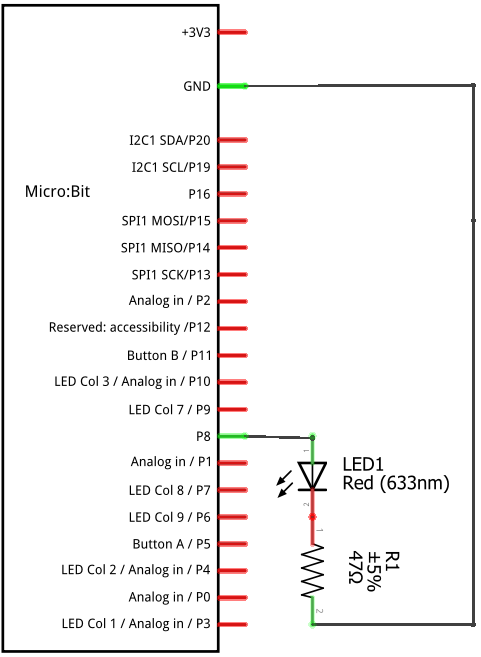
\includegraphics[width=0.65\textwidth]{figuren/externeLedCr}
			\caption{Een externe led aangesloten op P08 }
			\label{fig:exLd}
			
		\end{subfigure}
		\begin{subfigure}[b]{0.46\textwidth}
\begin{lstlisting}[caption={Het aansturen van een externe LED.},label={lst:extLd1}]
const int externeLed = 8;
			
void setup() {
	pinMode(externeLed, OUTPUT);  
}
				
void loop() {
  digitalWrite(externeLed,HIGH);
  delay(500);
  digitalWrite(externeLed,LOW);
  delay(500); 
}
\end{lstlisting}
		\end{subfigure}
		\captionsetup{justification=centering}
		\caption{Het aansturen van een externe LED. }
		\label{fig:vbExtld}
	\end{center}	
\end{figure}

De werking van het programma is als volgt.
\begin{enumerate}
	\item In de \textcolor{arduinoGreen}{setup}() wordt dit poortnummer op output gezet,\\  (\textcolor{arduinoOrange}	{pinMode} (externeLed,  \textcolor{arduinoBlue}{OUTPUT})); 
\item In de \textcolor{arduinoGreen}{loop}() wordt:
\begin{enumerate}
	\item Een spanning gezet op poort 8 (\textcolor{arduinoOrange}{digitalWrite}(externeLed, \textcolor{arduinoBlue}{HIGH});) waardoor een elektrische stroom door de LED gaat lopen en deze licht gaat geven. 
	\item Hierna wordt een halve seconde gewacht.
	\item Daarna wordt op poort 8,  0 Volt gezet (\textcolor{arduinoOrange}{digitalWrite}(externeLed, \textcolor{arduinoBlue}{LOW});) en gaat de LED uit (er loopt geen elektrische stroom meer door de LED).
		\item Hierna wordt een halve seconde gewacht.
\end{enumerate} 
\end{enumerate}
 
\subsection{Werken met de LED matrix}

Bij het blink programma in Listing \ref{lst:blink} wordt een LED aangestuurd dat een onderdeel is van de LED-matrix. De aangestuurde LED \textcolor{blue}{D2} is aangesloten op de pinnen \textcolor{green}{4} en \textcolor{green}{21}  aansluitingen van de LED-matrix wordt in figuur \ref{fig:ledmtx2} weergegeven.


\begin{minipage}{\linewidth}
	\begin{wrapfigure}[23]{r}{0.6\textwidth}
		\vspace{-15pt}
		\begin{center}
			\centering
			\captionsetup{justification=centering}
			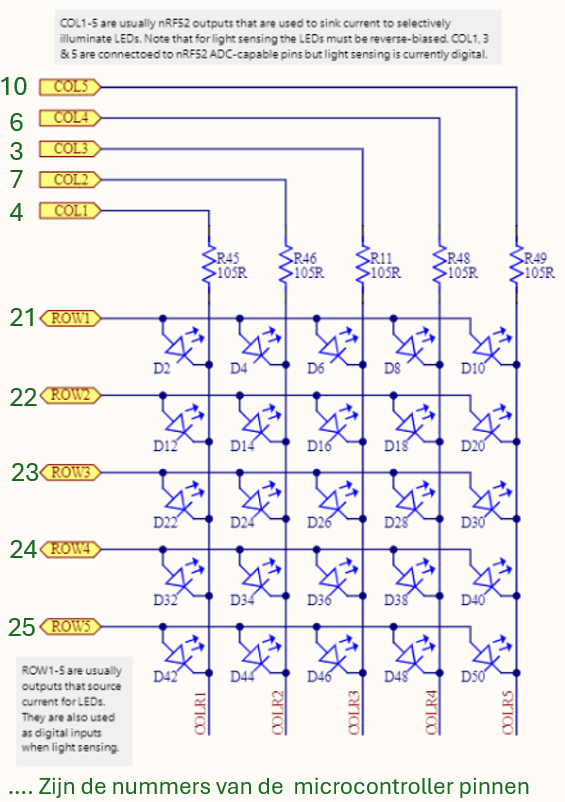
\includegraphics[width=0.45\textwidth]{figuren/LedMatrixV2Mnr}
		\end{center}
		%	\vspace{-14pt}
		\caption{Aansluitingen van de LED matrix..}
		\label{fig:ledmtx2}
	\end{wrapfigure}
	
~\vspace{2mm}\\
	Om de LED  (\img{figuren/diodeIc.png}) D2 aan te zetten, zou een elektrische stroom moeten lopen van  pin  \textcolor {Green}{21} door LED D2 naar pin \textcolor{Green}{4}.
	Dit kan voor elkaar verkregen worden door als eerst beide pinnen op output te zetten:\\
	\lstinline|	pinMode(4, OUTPUT);|\\ \lstinline|	pinMode(21, OUTPUT);|\\
	Vervolgens wordt pin \textcolor {Green}{4} laag gemaakt:\\
	 \lstinline|digitalWrite(4,LOW);|\\ en pin \textcolor {Green}{21} hoog gemaakt\\ \lstinline|digitalWrite(21,HIGH);|.\\
	 Indien pin \textcolor {Green}{21}  na een tijdje\\ \lstinline|delay(500);| weer laag wordt gemaakt\\ \lstinline|digitalWrite(21,LOW);| zal de LED uitgaan.
\end{minipage}


\subsection{Het aanzetten van meerdere ledjes in de matrix.}

\begin{enumerate}
	
\item In het programma \textit{blink} van listing \ref{lst:blink} knippert de LED met een frequentie van 1 Hz ($\frac{1}{2}$ seconde aan en $\frac{1}{2}$ seconde uit).\\
\begin{enumerate}
	\item Wijzig in de schets de eerste \textcolor{BurntOrange}{delay}(500) (regel 17) naar \textcolor{BurntOrange}{delay}(100).
	\item   Klik op \img{figuren/ardIcUpl.png} of druk \colorbox{mygray}{\textbf{Ctrl + U}} om het programma te compileren en naar de Microbit te sturen.
\end{enumerate}

Je ziet nu dat de ‘aan’ tijd langer is.
\item Laat nu ook LED D6 mee Knipperen (LED D2 en D6 knipperen).

\item Laat nu de LEDs D2 en D12 knipperen.

\item Laat nu de LEDs D2, D6 en D12.\\ 
\texttt{Verklaar wat er gebeurt}


%\item Laad nu ook LED D14 mee knipperen. (LED D2, D6, D12 en D14 Knipperen).\\ %\texttt{Verklaar wat er gebeurt}

\end{enumerate}

\section{De matrix programmeren met behulp van de Adafruit library}\label{sec:matrix}

De firma Adafruit heeft voor de micro:bit een library gemaakt waarin de LED matrix een component is, hierbij worden 5 getallen gebruikt die elk een rij voorstelt. Verder zijn er verschillende methode (functies) die gebruikt kunnen kunnen worden.

De belangrijkste methoden van de Adafruit\textunderscore Microbit\textunderscore Matrix bibliotheek zijn:
\begin{itemize}
	\item begin() om de matrix te initialiseren.
	\item clear() om alle LED's uit te zetten.
	\item drawPixel() om specifieke pixels aan of uit te zetten.
	\item writeDisplay() om de wijzigingen zichtbaar te maken.
	\item drawBitmap() om afbeeldingen weer te geven.
	\item print() om tekst op de matrix te tonen.
\end{itemize}

In Listing \ref{lst:ledmtx} wordt een voorbeeld gegeven van het gebruik van de Adafruit\_Microbit\_Matrix component.

\begin{lstlisting}[caption= Een LED matrix demo,label={lst:ledmtx},firstnumber=1]		
#include <Adafruit_Microbit.h>
Adafruit_Microbit_Matrix ledDisplay;  //definieer de led display

uint8_t led_matrix[] =
{ B00001, // bovenste rij met waarde 1.
	B00010,  //tweede rij  met waarde 2.
	B00100,  //derde rij  met waarde 4.
	8,       //vierde rij  met waarde B01000
	0x10,    //onderste rij met waarde B10000  of terwijl 16
};
void setup() {
	ledDisplay.begin(); 
	ledDisplay.drawPixel(2, 3, 1);  // Zet de LED op positie (2, 3) aan.
	delay(2000);  
	ledDisplay.clear();  
	delay(2000);  
	ledDisplay.show(led_matrix);
}
void loop() {
}
\end{lstlisting}

\paragraph{Opdracht: }Pas listing \ref{lst:ledmtx} zodanig aan, zodat alleen de LEDs D2, D6 en D21 knipperen.


\section{Het gebruik van de seriële poort.}

Je kunt de seriële poort gebruiken om informatie te verzenden of te ontvangen van je laptop b.v. om te ‘debuggen’, oftewel controleren of je programma doet wat je er van verwacht. In The Challenge kun je het gebruiken om sensordata naar je PC te sturen.In het voorbeeldprogramma van Listing \ref{lst:serial} wordt de waarde van de teller steeds over de seriële lijn verstuurd.

\begin{lstlisting}[caption= Een LED matrix demo,label={lst:serial},firstnumber=1]		
	
void setup() {
	Serial.begin(9600);
	Serial.println("start");
}
int teller=0;

void loop() {
	Serial.println(teller);
	delay(1000);
	teller++;
}
\end{lstlisting}


Open de seriële monitor(Tools$\rightarrow$Serial Monitor) of (druk \colorbox{mygray}{\textbf{Ctrl + Shift + M}}) of klik op \img{figuren/ardIcMo.png}. DE monitor verschijn op de output, zoals te zien is in figuur \ref{fig:arser}
\begin{figure}[H]
	\captionsetup{justification=centering}
	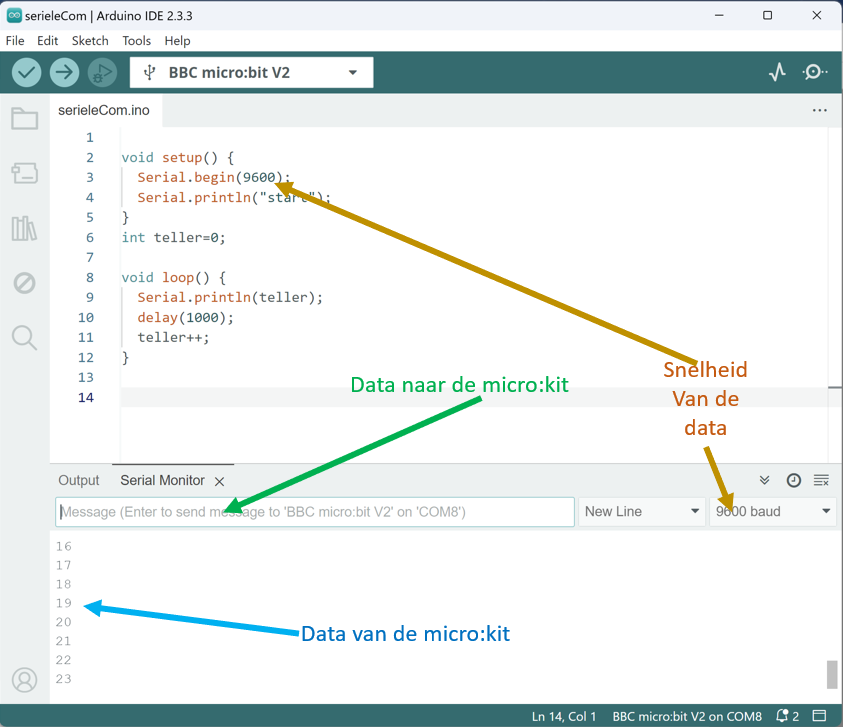
\includegraphics[width=0.5 \linewidth]{figuren/serial}
	\centering
	\caption{Instellingen van de seriële monitor.}
	\label{fig:arser}
\end{figure}
De instellingen van de monitor kan gedaan worden in de statusbalk, zoals te zien is in figuur \ref{fig:arser}.
Vaak wordt 9600 Baud (bits per seconde) gebruikt. Dit is gedaan omdat hiermee de data praktisch altijd stabiel verzonden wordt.

Zorg dat de ingestelde snelheid overeen komt met de instelling \textcolor{BurntOrange}{Serial.begin}(9600) in  \textcolor{OliveGreen}{setup}(). 

%Het programma in Listing \ref{lst:serial}  drukt de waarde van de teller af.\\

\paragraph{Opdracht Seriële communicatie:} 
Lees via de seriële poort een getal in en laat een LED het aantal keren knipperen zoals het ingelezen getal. Lees hierna opnieuw een getal in, etc...
\begin{figure}[H]
	\captionsetup{justification=centering}
	\centering
	\eerstefc

	\caption{De LED knippert x keer.}
	\label{fig:flowchart1}
\end{figure}
De flowchart van dit programma wordt weergegeven in figuur \ref{fig:flowchart1}

\paragraph{Opdracht Het binaire getal:} 
Bij deze opdracht wordt een random getal tussen de 0 en de 31 gekozen, die vervolgens op de middelste rij van de led-matrix geplaatst wordt. De gebruiker moet binnen 10 seconden raden wat het getal is. De flowchart van het programma wordt in figuur \ref{fig:flowchart2} weergegeven.
\begin{figure}[H]
	\captionsetup{justification=centering}
	\centering
	\randomfc
	
	\caption{Het raden van de binaire waarde.}
	\label{fig:flowchart2}
\end{figure}

